\documentclass[12pt,a4paper]{article}
\usepackage[utf8]{inputenc}
\usepackage[T1]{fontenc}
\usepackage[italian]{babel}
\usepackage{graphicx}
\usepackage{float}
\usepackage{geometry}
\usepackage{caption}
\usepackage{subcaption}
\usepackage{array}
\usepackage{longtable}
\usepackage{booktabs}
\usepackage{enumitem}

\geometry{
    left=2cm,
    right=2cm,
    top=2cm,
    bottom=2cm
}

\title{Diagrammi dei Casi d'Uso --- BugBoard26}
\author{Documentazione Progetto}
\date{\today}

\begin{document}

\maketitle

\begin{abstract}
Questo documento presenta i diagrammi dei casi d'uso per l'applicazione BugBoard26, sistema di tracciamento e gestione delle segnalazioni di bug, seguiti dalla formalizzazione dettagliata dei casi d'uso più significativi secondo il formalismo di Alistair Cockburn.
\end{abstract}

\tableofcontents
\newpage

% ============================================================
\section{Diagrammi dei Casi d'Uso}
% ============================================================

\subsection{Diagramma Generale del Sistema}
\begin{figure}[H]
    \centering
    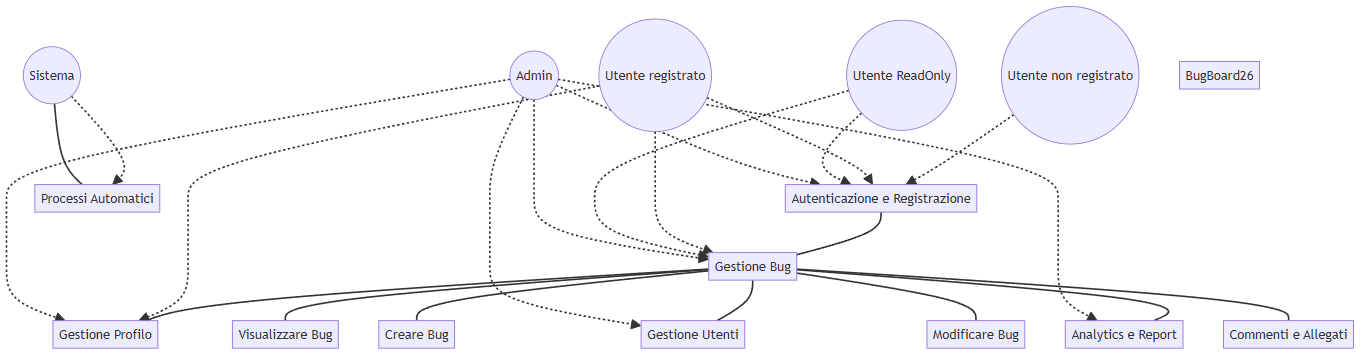
\includegraphics[width=0.85\textwidth]{immagini/diagramma_generale.png}
    \caption{Diagramma generale dei casi d'uso per BugBoard26}
    \label{fig:generale}
\end{figure}

Il diagramma generale mostra tutti gli attori del sistema e le loro interazioni con i casi d'uso principali:
\begin{itemize}
    \item \textbf{Attori}: Utente non registrato, Utente registrato (USER), Utente ReadOnly, Admin, Sistema
    \item \textbf{Gruppi di funzionalità}: Autenticazione, Gestione Bug, Gestione Profilo, Amministrazione
\end{itemize}

\subsection{Diagramma Dettagliato --- Gestione Bug}
\begin{figure}[H]
    \centering
    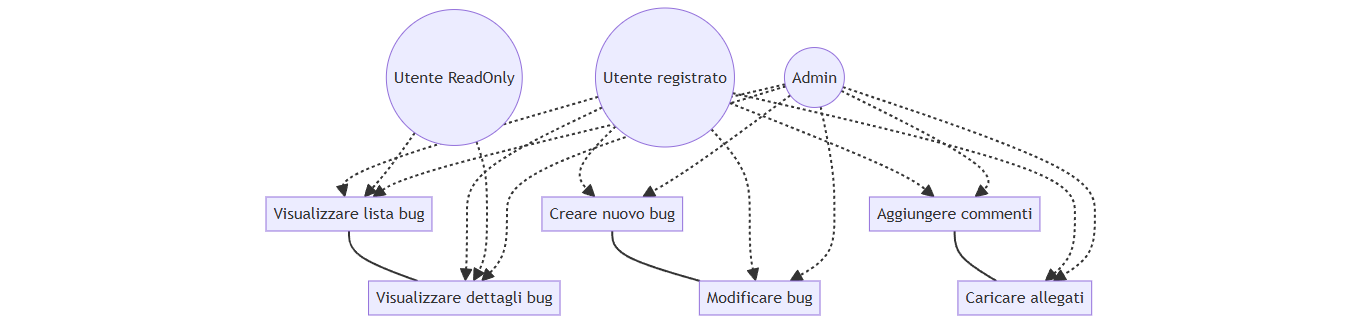
\includegraphics[width=0.85\textwidth]{immagini/diagramma_bug_management.png}
    \caption{Diagramma dettagliato delle operazioni di gestione bug}
    \label{fig:bug_management}
\end{figure}

Il diagramma si focalizza sulle operazioni specifiche di gestione dei bug:
\begin{itemize}
    \item \textbf{Operazioni}: Visualizzare, creare, modificare, archiviare bug
    \item \textbf{Funzionalità aggiuntive}: Commenti, allegati immagini, filtri di ricerca
    \item \textbf{Differenze per ruolo}: Utente ReadOnly può solo leggere; Admin ha accesso completo
\end{itemize}

\subsection{Diagramma Dettagliato --- Amministrazione}
\begin{figure}[H]
    \centering
    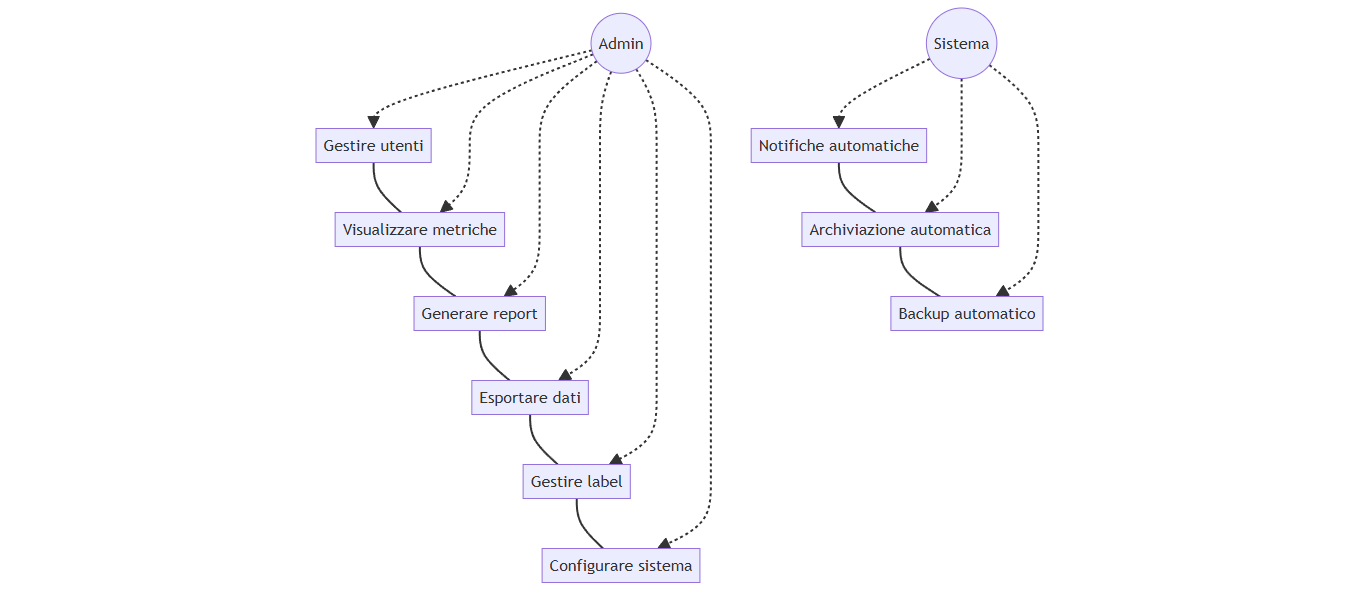
\includegraphics[width=0.85\textwidth]{immagini/diagramma_amministrazione.png}
    \caption{Diagramma dettagliato delle funzionalità di amministrazione}
    \label{fig:amministrazione}
\end{figure}

\subsection{Convenzioni Grafiche}
\begin{itemize}
    \item \textbf{Attori} (omino/rettangolo): Utenti o sistemi esterni che interagiscono con BugBoard26
    \item \textbf{Casi d'uso} (ellissi): Funzionalità del sistema
    \item \textbf{Linee solide}: Associazione --- l'attore partecipa al caso d'uso
    \item \textbf{Linee tratteggiate $\ll$include$\gg$}: Inclusione obbligatoria di un altro caso d'uso
    \item \textbf{Linee tratteggiate $\ll$extend$\gg$}: Estensione opzionale di un caso d'uso
\end{itemize}

% ============================================================
\section{Casi d'Uso Dettagliati (Formalismo Cockburn)}
% ============================================================

% I casi d'uso dettagliati sono definiti nel file casi_uso_dettagliati.tex
% ============================================================
% CORPO: Casi d'Uso Dettagliati (Formalismo Cockburn)
% Questo file va incluso con % ============================================================
% CORPO: Casi d'Uso Dettagliati (Formalismo Cockburn)
% Questo file va incluso con % ============================================================
% CORPO: Casi d'Uso Dettagliati (Formalismo Cockburn)
% Questo file va incluso con \input{casi_uso_dettagliati_body}
% ============================================================

\subsection{Caso d'Uso 1: Creazione nuovo bug}

\begin{longtable}{|p{3cm}|p{7cm}|p{5.5cm}|}
\hline
\textbf{Campo} & \multicolumn{2}{p{12.5cm}|}{\textbf{Descrizione}} \\
\hline
\endfirsthead
\hline
\textbf{Campo} & \multicolumn{2}{p{12.5cm}|}{\textbf{Descrizione}} \\
\hline
\endhead
\hline
\endfoot
\hline
\endlastfoot

USE CASE \#01 & \multicolumn{2}{p{12.5cm}|}{CREAZIONE NUOVO BUG} \\
\hline
Goal & \multicolumn{2}{p{12.5cm}|}{L'utente vuole segnalare un nuovo bug nel sistema} \\
\hline
Preconditions & \multicolumn{2}{p{12.5cm}|}{L'utente deve essere autenticato (ruolo USER o ADMIN)} \\
\hline
Success End Condition & \multicolumn{2}{p{12.5cm}|}{Il bug è creato con successo e registrato con un ID univoco} \\
\hline
Failed End Condition & \multicolumn{2}{p{12.5cm}|}{Il bug non viene creato a causa di errori di validazione o problemi di sistema} \\
\hline
Primary Actor & \multicolumn{2}{p{12.5cm}|}{Utente registrato (USER)} \\
\hline\hline
\textbf{DESCRIPTION} & \textbf{Utente} & \textbf{Sistema} \\
\hline
Step 1 & Accede alla sezione ``Nuovo Bug'' & Mostra il form con i campi obbligatori \\
\hline
Step 2 & Inserisce il titolo del bug & Valida che il titolo non sia vuoto \\
\hline
Step 3 & Seleziona il tipo (Bug, Feature, Enhancement) & Carica le categorie disponibili \\
\hline
Step 4 & Inserisce la descrizione dettagliata & Fornisce un'area di testo \\
\hline
Step 5 & Seleziona la priorità (Low, Medium, High, Critical) & Mostra le opzioni con colori identificativi \\
\hline
Step 6 & Aggiunge label/tag opzionali & Permette selezione multipla da lista \\
\hline
Step 7 & Carica immagini allegati (opzionale) & Valida formato (JPEG, PNG, GIF, WebP) e dimensione (max 5\,MB) \\
\hline
Step 8 & Seleziona assegnatario (opzionale) & Mostra lista utenti attivi \\
\hline
Step 9 & Clicca su ``Crea Bug'' & Valida tutti i campi obbligatori \\
\hline
Step 10 & & Salva il bug nel database \\
\hline
Step 11 & & Invia notifica all'utente assegnato (se presente) \\
\hline
Step 12 & & Mostra conferma con l'ID del bug creato \\
\hline\hline
\textbf{EXTENSIONS} & \textbf{Step} & \textbf{Descrizione} \\
\hline
Caricamento immagini fallito & 7.a & Mostra errore ``Formato non supportato'' \\
\hline
 & 7.b & L'utente può riprovare con file diverso \\
\hline
Validazione campi fallita & 9.a & Evidenzia i campi con errori \\
\hline
 & 9.b & Mostra messaggi di errore per ciascun campo \\
\hline
Utente assegnatario non trovato & 8.a & Mostra errore ``Utente non trovato'' \\
\hline
 & 8.b & L'utente può eseguire una nuova ricerca \\
\hline
\end{longtable}

% ============================================================
\subsection{Caso d'Uso 2: Assegnazione bug a un utente}

\begin{longtable}{|p{3cm}|p{7cm}|p{5.5cm}|}
\hline
\textbf{Campo} & \multicolumn{2}{p{12.5cm}|}{\textbf{Descrizione}} \\
\hline
\endfirsthead
\hline
\textbf{Campo} & \multicolumn{2}{p{12.5cm}|}{\textbf{Descrizione}} \\
\hline
\endhead
\hline
\endfoot
\hline
\endlastfoot

USE CASE \#02 & \multicolumn{2}{p{12.5cm}|}{ASSEGNAZIONE BUG A UN UTENTE} \\
\hline
Goal & \multicolumn{2}{p{12.5cm}|}{L'amministratore vuole assegnare o riassegnare un bug a un utente del sistema} \\
\hline
Preconditions & \multicolumn{2}{p{12.5cm}|}{L'utente deve essere autenticato con ruolo ADMIN; il bug deve esistere nel sistema} \\
\hline
Success End Condition & \multicolumn{2}{p{12.5cm}|}{Il bug risulta assegnato al nuovo utente e la modifica è registrata nello storico} \\
\hline
Failed End Condition & \multicolumn{2}{p{12.5cm}|}{L'assegnazione fallisce per utente di destinazione non valido} \\
\hline
Primary Actor & \multicolumn{2}{p{12.5cm}|}{Admin} \\
\hline\hline
\textbf{DESCRIPTION} & \textbf{Utente (Admin)} & \textbf{Sistema} \\
\hline
Step 1 & Visualizza i dettagli di un bug & Mostra la pagina di dettaglio con tutte le informazioni \\
\hline
Step 2 & Clicca su ``Assegna'' & Apre il form di assegnazione \\
\hline
Step 3 & Inserisce email o nome del nuovo assegnatario & Fornisce autocomplete con ricerca utenti \\
\hline
Step 4 & Seleziona l'utente dalla lista & Valida che l'utente esista e sia attivo \\
\hline
Step 5 & Aggiunge una nota (opzionale) & Fornisce un campo testo per la motivazione \\
\hline
Step 6 & Clicca su ``Conferma Assegnazione'' & Verifica i permessi dell'utente richiedente \\
\hline
Step 7 & & Aggiorna il campo ``assegnato a'' nel database \\
\hline
Step 8 & & Registra la modifica nella tabella history \\
\hline
Step 9 & & Invia notifica al nuovo assegnatario \\
\hline
Step 10 & & Invia notifica all'assegnatario precedente (se diverso) \\
\hline
Step 11 & & Mostra messaggio di conferma \\
\hline\hline
\textbf{EXTENSIONS} & \textbf{Step} & \textbf{Descrizione} \\
\hline
Utente non trovato & 4.a & Mostra errore ``Utente non esistente'' \\
\hline
 & 4.b & L'admin può eseguire una nuova ricerca \\
\hline
Bug già assegnato & 6.a & Chiede conferma per il cambio di assegnazione \\
\hline
 & 6.b & Se confermato, procede con la riassegnazione \\
\hline
\end{longtable}

% ============================================================
\subsection{Caso d'Uso 3: Risoluzione e chiusura bug}

\begin{longtable}{|p{3cm}|p{7cm}|p{5.5cm}|}
\hline
\textbf{Campo} & \multicolumn{2}{p{12.5cm}|}{\textbf{Descrizione}} \\
\hline
\endfirsthead
\hline
\textbf{Campo} & \multicolumn{2}{p{12.5cm}|}{\textbf{Descrizione}} \\
\hline
\endhead
\hline
\endfoot
\hline
\endlastfoot

USE CASE \#03 & \multicolumn{2}{p{12.5cm}|}{RISOLUZIONE E CHIUSURA BUG} \\
\hline
Goal & \multicolumn{2}{p{12.5cm}|}{L'utente vuole marcare un bug come risolto} \\
\hline
Preconditions & \multicolumn{2}{p{12.5cm}|}{L'utente deve essere autenticato e assegnatario del bug; il bug deve essere in stato \textit{In Progress}} \\
\hline
Success End Condition & \multicolumn{2}{p{12.5cm}|}{Il bug viene aggiornato allo stato \textit{Resolved} con data di risoluzione registrata} \\
\hline
Failed End Condition & \multicolumn{2}{p{12.5cm}|}{La risoluzione fallisce per permessi insufficienti o stato del bug non valido} \\
\hline
Primary Actor & \multicolumn{2}{p{12.5cm}|}{Utente registrato (USER) assegnato al bug} \\
\hline\hline
\textbf{DESCRIPTION} & \textbf{Utente} & \textbf{Sistema} \\
\hline
Step 1 & Visualizza i dettagli del bug assegnato & Mostra la pagina di dettaglio con lo stato attuale \\
\hline
Step 2 & Clicca su ``Risolvi Bug'' & Verifica che il bug sia in stato \textit{In Progress} \\
\hline
Step 3 & & Mostra il form di risoluzione \\
\hline
Step 4 & Seleziona il tipo di risoluzione & Mostra opzioni: \textit{Fixed, Won't Fix, Duplicate, Cannot Reproduce} \\
\hline
Step 5 & Inserisce la descrizione della soluzione adottata & Fornisce un'area di testo \\
\hline
Step 6 & Carica immagini di conferma (opzionale) & Valida formato e dimensione degli allegati \\
\hline
Step 7 & Clicca su ``Conferma Risoluzione'' & Valida tutti i campi obbligatori \\
\hline
Step 8 & & Aggiorna lo stato a \textit{Resolved} \\
\hline
Step 9 & & Registra la data di risoluzione \\
\hline
Step 10 & & Crea un record nella tabella history \\
\hline
Step 11 & & Invia notifiche al creatore e ai follower del bug \\
\hline
Step 12 & & Mostra la pagina aggiornata con il nuovo stato \\
\hline\hline
\textbf{EXTENSIONS} & \textbf{Step} & \textbf{Descrizione} \\
\hline
Bug non in stato corretto & 2.a & Mostra ``Bug non può essere risolto in questo stato'' \\
\hline
 & 2.b & Suggerisce azioni alternative disponibili \\
\hline
Tipo risoluzione ``Duplicate'' & 4.a & Richiede la selezione del bug padre \\
\hline
 & 4.b & Crea automaticamente la relazione di duplicazione \\
\hline
Caricamento immagini fallito & 6.a & Mostra errore di formato o dimensione \\
\hline
 & 6.b & L'utente può proseguire senza allegati \\
\hline
\end{longtable}

% ============================================================
\subsection{Caso d'Uso 4: Generazione report mensile (Admin)}

\begin{longtable}{|p{3cm}|p{7cm}|p{5.5cm}|}
\hline
\textbf{Campo} & \multicolumn{2}{p{12.5cm}|}{\textbf{Descrizione}} \\
\hline
\endfirsthead
\hline
\textbf{Campo} & \multicolumn{2}{p{12.5cm}|}{\textbf{Descrizione}} \\
\hline
\endhead
\hline
\endfoot
\hline
\endlastfoot

USE CASE \#04 & \multicolumn{2}{p{12.5cm}|}{GENERAZIONE REPORT MENSILE} \\
\hline
Goal & \multicolumn{2}{p{12.5cm}|}{L'amministratore vuole generare un report sull'attività del sistema per un mese specifico} \\
\hline
Preconditions & \multicolumn{2}{p{12.5cm}|}{L'utente deve essere autenticato con ruolo ADMIN} \\
\hline
Success End Condition & \multicolumn{2}{p{12.5cm}|}{Il report viene generato e reso disponibile per il download} \\
\hline
Failed End Condition & \multicolumn{2}{p{12.5cm}|}{La generazione fallisce per assenza di dati nel periodo selezionato o errori di sistema} \\
\hline
Primary Actor & \multicolumn{2}{p{12.5cm}|}{Admin} \\
\hline\hline
\textbf{DESCRIPTION} & \textbf{Utente (Admin)} & \textbf{Sistema} \\
\hline
Step 1 & Accede alla sezione ``Analytics'' & Mostra la dashboard con le opzioni di reportistica \\
\hline
Step 2 & Seleziona ``Report Mensili'' & Carica la lista dei mesi disponibili \\
\hline
Step 3 & Seleziona mese e anno desiderati & Valida che il periodo esista e contenga dati \\
\hline
Step 4 & Clicca su ``Genera Report'' & Avvia il processo di generazione \\
\hline
Step 5 & & Raccoglie dati dalle tabelle bugs, users, history \\
\hline
Step 6 & & Calcola metriche: bug creati, risolti, tempo medio \\
\hline
Step 7 & & Genera grafici e statistiche aggregate \\
\hline
Step 8 & & Crea il documento in formato Excel \\
\hline
Step 9 & & Fornisce il link per il download \\
\hline
Step 10 & Scarica il report & Serve il file con nome che include il timestamp \\
\hline\hline
\textbf{EXTENSIONS} & \textbf{Step} & \textbf{Descrizione} \\
\hline
Mese senza dati & 3.a & Avvisa ``Nessun dato disponibile per il periodo selezionato'' \\
\hline
 & 3.b & Suggerisce periodi alternativi \\
\hline
Errore generazione & 8.a & Registra l'errore nel log \\
\hline
 & 8.b & Mostra un messaggio di errore all'amministratore \\
\hline
 & 8.c & Suggerisce di riprovare o contattare il supporto \\
\hline
\end{longtable}

% ============================================================

\subsection{Caso d'Uso 1: Creazione nuovo bug}

\begin{longtable}{|p{3cm}|p{7cm}|p{5.5cm}|}
\hline
\textbf{Campo} & \multicolumn{2}{p{12.5cm}|}{\textbf{Descrizione}} \\
\hline
\endfirsthead
\hline
\textbf{Campo} & \multicolumn{2}{p{12.5cm}|}{\textbf{Descrizione}} \\
\hline
\endhead
\hline
\endfoot
\hline
\endlastfoot

USE CASE \#01 & \multicolumn{2}{p{12.5cm}|}{CREAZIONE NUOVO BUG} \\
\hline
Goal & \multicolumn{2}{p{12.5cm}|}{L'utente vuole segnalare un nuovo bug nel sistema} \\
\hline
Preconditions & \multicolumn{2}{p{12.5cm}|}{L'utente deve essere autenticato (ruolo USER o ADMIN)} \\
\hline
Success End Condition & \multicolumn{2}{p{12.5cm}|}{Il bug è creato con successo e registrato con un ID univoco} \\
\hline
Failed End Condition & \multicolumn{2}{p{12.5cm}|}{Il bug non viene creato a causa di errori di validazione o problemi di sistema} \\
\hline
Primary Actor & \multicolumn{2}{p{12.5cm}|}{Utente registrato (USER)} \\
\hline\hline
\textbf{DESCRIPTION} & \textbf{Utente} & \textbf{Sistema} \\
\hline
Step 1 & Accede alla sezione ``Nuovo Bug'' & Mostra il form con i campi obbligatori \\
\hline
Step 2 & Inserisce il titolo del bug & Valida che il titolo non sia vuoto \\
\hline
Step 3 & Seleziona il tipo (Bug, Feature, Enhancement) & Carica le categorie disponibili \\
\hline
Step 4 & Inserisce la descrizione dettagliata & Fornisce un'area di testo \\
\hline
Step 5 & Seleziona la priorità (Low, Medium, High, Critical) & Mostra le opzioni con colori identificativi \\
\hline
Step 6 & Aggiunge label/tag opzionali & Permette selezione multipla da lista \\
\hline
Step 7 & Carica immagini allegati (opzionale) & Valida formato (JPEG, PNG, GIF, WebP) e dimensione (max 5\,MB) \\
\hline
Step 8 & Seleziona assegnatario (opzionale) & Mostra lista utenti attivi \\
\hline
Step 9 & Clicca su ``Crea Bug'' & Valida tutti i campi obbligatori \\
\hline
Step 10 & & Salva il bug nel database \\
\hline
Step 11 & & Invia notifica all'utente assegnato (se presente) \\
\hline
Step 12 & & Mostra conferma con l'ID del bug creato \\
\hline\hline
\textbf{EXTENSIONS} & \textbf{Step} & \textbf{Descrizione} \\
\hline
Caricamento immagini fallito & 7.a & Mostra errore ``Formato non supportato'' \\
\hline
 & 7.b & L'utente può riprovare con file diverso \\
\hline
Validazione campi fallita & 9.a & Evidenzia i campi con errori \\
\hline
 & 9.b & Mostra messaggi di errore per ciascun campo \\
\hline
Utente assegnatario non trovato & 8.a & Mostra errore ``Utente non trovato'' \\
\hline
 & 8.b & L'utente può eseguire una nuova ricerca \\
\hline
\end{longtable}

% ============================================================
\subsection{Caso d'Uso 2: Assegnazione bug a un utente}

\begin{longtable}{|p{3cm}|p{7cm}|p{5.5cm}|}
\hline
\textbf{Campo} & \multicolumn{2}{p{12.5cm}|}{\textbf{Descrizione}} \\
\hline
\endfirsthead
\hline
\textbf{Campo} & \multicolumn{2}{p{12.5cm}|}{\textbf{Descrizione}} \\
\hline
\endhead
\hline
\endfoot
\hline
\endlastfoot

USE CASE \#02 & \multicolumn{2}{p{12.5cm}|}{ASSEGNAZIONE BUG A UN UTENTE} \\
\hline
Goal & \multicolumn{2}{p{12.5cm}|}{L'amministratore vuole assegnare o riassegnare un bug a un utente del sistema} \\
\hline
Preconditions & \multicolumn{2}{p{12.5cm}|}{L'utente deve essere autenticato con ruolo ADMIN; il bug deve esistere nel sistema} \\
\hline
Success End Condition & \multicolumn{2}{p{12.5cm}|}{Il bug risulta assegnato al nuovo utente e la modifica è registrata nello storico} \\
\hline
Failed End Condition & \multicolumn{2}{p{12.5cm}|}{L'assegnazione fallisce per utente di destinazione non valido} \\
\hline
Primary Actor & \multicolumn{2}{p{12.5cm}|}{Admin} \\
\hline\hline
\textbf{DESCRIPTION} & \textbf{Utente (Admin)} & \textbf{Sistema} \\
\hline
Step 1 & Visualizza i dettagli di un bug & Mostra la pagina di dettaglio con tutte le informazioni \\
\hline
Step 2 & Clicca su ``Assegna'' & Apre il form di assegnazione \\
\hline
Step 3 & Inserisce email o nome del nuovo assegnatario & Fornisce autocomplete con ricerca utenti \\
\hline
Step 4 & Seleziona l'utente dalla lista & Valida che l'utente esista e sia attivo \\
\hline
Step 5 & Aggiunge una nota (opzionale) & Fornisce un campo testo per la motivazione \\
\hline
Step 6 & Clicca su ``Conferma Assegnazione'' & Verifica i permessi dell'utente richiedente \\
\hline
Step 7 & & Aggiorna il campo ``assegnato a'' nel database \\
\hline
Step 8 & & Registra la modifica nella tabella history \\
\hline
Step 9 & & Invia notifica al nuovo assegnatario \\
\hline
Step 10 & & Invia notifica all'assegnatario precedente (se diverso) \\
\hline
Step 11 & & Mostra messaggio di conferma \\
\hline\hline
\textbf{EXTENSIONS} & \textbf{Step} & \textbf{Descrizione} \\
\hline
Utente non trovato & 4.a & Mostra errore ``Utente non esistente'' \\
\hline
 & 4.b & L'admin può eseguire una nuova ricerca \\
\hline
Bug già assegnato & 6.a & Chiede conferma per il cambio di assegnazione \\
\hline
 & 6.b & Se confermato, procede con la riassegnazione \\
\hline
\end{longtable}

% ============================================================
\subsection{Caso d'Uso 3: Risoluzione e chiusura bug}

\begin{longtable}{|p{3cm}|p{7cm}|p{5.5cm}|}
\hline
\textbf{Campo} & \multicolumn{2}{p{12.5cm}|}{\textbf{Descrizione}} \\
\hline
\endfirsthead
\hline
\textbf{Campo} & \multicolumn{2}{p{12.5cm}|}{\textbf{Descrizione}} \\
\hline
\endhead
\hline
\endfoot
\hline
\endlastfoot

USE CASE \#03 & \multicolumn{2}{p{12.5cm}|}{RISOLUZIONE E CHIUSURA BUG} \\
\hline
Goal & \multicolumn{2}{p{12.5cm}|}{L'utente vuole marcare un bug come risolto} \\
\hline
Preconditions & \multicolumn{2}{p{12.5cm}|}{L'utente deve essere autenticato e assegnatario del bug; il bug deve essere in stato \textit{In Progress}} \\
\hline
Success End Condition & \multicolumn{2}{p{12.5cm}|}{Il bug viene aggiornato allo stato \textit{Resolved} con data di risoluzione registrata} \\
\hline
Failed End Condition & \multicolumn{2}{p{12.5cm}|}{La risoluzione fallisce per permessi insufficienti o stato del bug non valido} \\
\hline
Primary Actor & \multicolumn{2}{p{12.5cm}|}{Utente registrato (USER) assegnato al bug} \\
\hline\hline
\textbf{DESCRIPTION} & \textbf{Utente} & \textbf{Sistema} \\
\hline
Step 1 & Visualizza i dettagli del bug assegnato & Mostra la pagina di dettaglio con lo stato attuale \\
\hline
Step 2 & Clicca su ``Risolvi Bug'' & Verifica che il bug sia in stato \textit{In Progress} \\
\hline
Step 3 & & Mostra il form di risoluzione \\
\hline
Step 4 & Seleziona il tipo di risoluzione & Mostra opzioni: \textit{Fixed, Won't Fix, Duplicate, Cannot Reproduce} \\
\hline
Step 5 & Inserisce la descrizione della soluzione adottata & Fornisce un'area di testo \\
\hline
Step 6 & Carica immagini di conferma (opzionale) & Valida formato e dimensione degli allegati \\
\hline
Step 7 & Clicca su ``Conferma Risoluzione'' & Valida tutti i campi obbligatori \\
\hline
Step 8 & & Aggiorna lo stato a \textit{Resolved} \\
\hline
Step 9 & & Registra la data di risoluzione \\
\hline
Step 10 & & Crea un record nella tabella history \\
\hline
Step 11 & & Invia notifiche al creatore e ai follower del bug \\
\hline
Step 12 & & Mostra la pagina aggiornata con il nuovo stato \\
\hline\hline
\textbf{EXTENSIONS} & \textbf{Step} & \textbf{Descrizione} \\
\hline
Bug non in stato corretto & 2.a & Mostra ``Bug non può essere risolto in questo stato'' \\
\hline
 & 2.b & Suggerisce azioni alternative disponibili \\
\hline
Tipo risoluzione ``Duplicate'' & 4.a & Richiede la selezione del bug padre \\
\hline
 & 4.b & Crea automaticamente la relazione di duplicazione \\
\hline
Caricamento immagini fallito & 6.a & Mostra errore di formato o dimensione \\
\hline
 & 6.b & L'utente può proseguire senza allegati \\
\hline
\end{longtable}

% ============================================================
\subsection{Caso d'Uso 4: Generazione report mensile (Admin)}

\begin{longtable}{|p{3cm}|p{7cm}|p{5.5cm}|}
\hline
\textbf{Campo} & \multicolumn{2}{p{12.5cm}|}{\textbf{Descrizione}} \\
\hline
\endfirsthead
\hline
\textbf{Campo} & \multicolumn{2}{p{12.5cm}|}{\textbf{Descrizione}} \\
\hline
\endhead
\hline
\endfoot
\hline
\endlastfoot

USE CASE \#04 & \multicolumn{2}{p{12.5cm}|}{GENERAZIONE REPORT MENSILE} \\
\hline
Goal & \multicolumn{2}{p{12.5cm}|}{L'amministratore vuole generare un report sull'attività del sistema per un mese specifico} \\
\hline
Preconditions & \multicolumn{2}{p{12.5cm}|}{L'utente deve essere autenticato con ruolo ADMIN} \\
\hline
Success End Condition & \multicolumn{2}{p{12.5cm}|}{Il report viene generato e reso disponibile per il download} \\
\hline
Failed End Condition & \multicolumn{2}{p{12.5cm}|}{La generazione fallisce per assenza di dati nel periodo selezionato o errori di sistema} \\
\hline
Primary Actor & \multicolumn{2}{p{12.5cm}|}{Admin} \\
\hline\hline
\textbf{DESCRIPTION} & \textbf{Utente (Admin)} & \textbf{Sistema} \\
\hline
Step 1 & Accede alla sezione ``Analytics'' & Mostra la dashboard con le opzioni di reportistica \\
\hline
Step 2 & Seleziona ``Report Mensili'' & Carica la lista dei mesi disponibili \\
\hline
Step 3 & Seleziona mese e anno desiderati & Valida che il periodo esista e contenga dati \\
\hline
Step 4 & Clicca su ``Genera Report'' & Avvia il processo di generazione \\
\hline
Step 5 & & Raccoglie dati dalle tabelle bugs, users, history \\
\hline
Step 6 & & Calcola metriche: bug creati, risolti, tempo medio \\
\hline
Step 7 & & Genera grafici e statistiche aggregate \\
\hline
Step 8 & & Crea il documento in formato Excel \\
\hline
Step 9 & & Fornisce il link per il download \\
\hline
Step 10 & Scarica il report & Serve il file con nome che include il timestamp \\
\hline\hline
\textbf{EXTENSIONS} & \textbf{Step} & \textbf{Descrizione} \\
\hline
Mese senza dati & 3.a & Avvisa ``Nessun dato disponibile per il periodo selezionato'' \\
\hline
 & 3.b & Suggerisce periodi alternativi \\
\hline
Errore generazione & 8.a & Registra l'errore nel log \\
\hline
 & 8.b & Mostra un messaggio di errore all'amministratore \\
\hline
 & 8.c & Suggerisce di riprovare o contattare il supporto \\
\hline
\end{longtable}

% ============================================================

\subsection{Caso d'Uso 1: Creazione nuovo bug}

\begin{longtable}{|p{3cm}|p{7cm}|p{5.5cm}|}
\hline
\textbf{Campo} & \multicolumn{2}{p{12.5cm}|}{\textbf{Descrizione}} \\
\hline
\endfirsthead
\hline
\textbf{Campo} & \multicolumn{2}{p{12.5cm}|}{\textbf{Descrizione}} \\
\hline
\endhead
\hline
\endfoot
\hline
\endlastfoot

USE CASE \#01 & \multicolumn{2}{p{12.5cm}|}{CREAZIONE NUOVO BUG} \\
\hline
Goal & \multicolumn{2}{p{12.5cm}|}{L'utente vuole segnalare un nuovo bug nel sistema} \\
\hline
Preconditions & \multicolumn{2}{p{12.5cm}|}{L'utente deve essere autenticato (ruolo USER o ADMIN)} \\
\hline
Success End Condition & \multicolumn{2}{p{12.5cm}|}{Il bug è creato con successo e registrato con un ID univoco} \\
\hline
Failed End Condition & \multicolumn{2}{p{12.5cm}|}{Il bug non viene creato a causa di errori di validazione o problemi di sistema} \\
\hline
Primary Actor & \multicolumn{2}{p{12.5cm}|}{Utente registrato (USER)} \\
\hline\hline
\textbf{DESCRIPTION} & \textbf{Utente} & \textbf{Sistema} \\
\hline
Step 1 & Accede alla sezione ``Nuovo Bug'' & Mostra il form con i campi obbligatori \\
\hline
Step 2 & Inserisce il titolo del bug & Valida che il titolo non sia vuoto \\
\hline
Step 3 & Seleziona il tipo (Bug, Feature, Enhancement) & Carica le categorie disponibili \\
\hline
Step 4 & Inserisce la descrizione dettagliata & Fornisce un'area di testo \\
\hline
Step 5 & Seleziona la priorità (Low, Medium, High, Critical) & Mostra le opzioni con colori identificativi \\
\hline
Step 6 & Aggiunge label/tag opzionali & Permette selezione multipla da lista \\
\hline
Step 7 & Carica immagini allegati (opzionale) & Valida formato (JPEG, PNG, GIF, WebP) e dimensione (max 5\,MB) \\
\hline
Step 8 & Seleziona assegnatario (opzionale) & Mostra lista utenti attivi \\
\hline
Step 9 & Clicca su ``Crea Bug'' & Valida tutti i campi obbligatori \\
\hline
Step 10 & & Salva il bug nel database \\
\hline
Step 11 & & Invia notifica all'utente assegnato (se presente) \\
\hline
Step 12 & & Mostra conferma con l'ID del bug creato \\
\hline\hline
\textbf{EXTENSIONS} & \textbf{Step} & \textbf{Descrizione} \\
\hline
Caricamento immagini fallito & 7.a & Mostra errore ``Formato non supportato'' \\
\hline
 & 7.b & L'utente può riprovare con file diverso \\
\hline
Validazione campi fallita & 9.a & Evidenzia i campi con errori \\
\hline
 & 9.b & Mostra messaggi di errore per ciascun campo \\
\hline
Utente assegnatario non trovato & 8.a & Mostra errore ``Utente non trovato'' \\
\hline
 & 8.b & L'utente può eseguire una nuova ricerca \\
\hline
\end{longtable}

% ============================================================
\subsection{Caso d'Uso 2: Assegnazione bug a un utente}

\begin{longtable}{|p{3cm}|p{7cm}|p{5.5cm}|}
\hline
\textbf{Campo} & \multicolumn{2}{p{12.5cm}|}{\textbf{Descrizione}} \\
\hline
\endfirsthead
\hline
\textbf{Campo} & \multicolumn{2}{p{12.5cm}|}{\textbf{Descrizione}} \\
\hline
\endhead
\hline
\endfoot
\hline
\endlastfoot

USE CASE \#02 & \multicolumn{2}{p{12.5cm}|}{ASSEGNAZIONE BUG A UN UTENTE} \\
\hline
Goal & \multicolumn{2}{p{12.5cm}|}{L'amministratore vuole assegnare o riassegnare un bug a un utente del sistema} \\
\hline
Preconditions & \multicolumn{2}{p{12.5cm}|}{L'utente deve essere autenticato con ruolo ADMIN; il bug deve esistere nel sistema} \\
\hline
Success End Condition & \multicolumn{2}{p{12.5cm}|}{Il bug risulta assegnato al nuovo utente e la modifica è registrata nello storico} \\
\hline
Failed End Condition & \multicolumn{2}{p{12.5cm}|}{L'assegnazione fallisce per utente di destinazione non valido} \\
\hline
Primary Actor & \multicolumn{2}{p{12.5cm}|}{Admin} \\
\hline\hline
\textbf{DESCRIPTION} & \textbf{Utente (Admin)} & \textbf{Sistema} \\
\hline
Step 1 & Visualizza i dettagli di un bug & Mostra la pagina di dettaglio con tutte le informazioni \\
\hline
Step 2 & Clicca su ``Assegna'' & Apre il form di assegnazione \\
\hline
Step 3 & Inserisce email o nome del nuovo assegnatario & Fornisce autocomplete con ricerca utenti \\
\hline
Step 4 & Seleziona l'utente dalla lista & Valida che l'utente esista e sia attivo \\
\hline
Step 5 & Aggiunge una nota (opzionale) & Fornisce un campo testo per la motivazione \\
\hline
Step 6 & Clicca su ``Conferma Assegnazione'' & Verifica i permessi dell'utente richiedente \\
\hline
Step 7 & & Aggiorna il campo ``assegnato a'' nel database \\
\hline
Step 8 & & Registra la modifica nella tabella history \\
\hline
Step 9 & & Invia notifica al nuovo assegnatario \\
\hline
Step 10 & & Invia notifica all'assegnatario precedente (se diverso) \\
\hline
Step 11 & & Mostra messaggio di conferma \\
\hline\hline
\textbf{EXTENSIONS} & \textbf{Step} & \textbf{Descrizione} \\
\hline
Utente non trovato & 4.a & Mostra errore ``Utente non esistente'' \\
\hline
 & 4.b & L'admin può eseguire una nuova ricerca \\
\hline
Bug già assegnato & 6.a & Chiede conferma per il cambio di assegnazione \\
\hline
 & 6.b & Se confermato, procede con la riassegnazione \\
\hline
\end{longtable}

% ============================================================
\subsection{Caso d'Uso 3: Risoluzione e chiusura bug}

\begin{longtable}{|p{3cm}|p{7cm}|p{5.5cm}|}
\hline
\textbf{Campo} & \multicolumn{2}{p{12.5cm}|}{\textbf{Descrizione}} \\
\hline
\endfirsthead
\hline
\textbf{Campo} & \multicolumn{2}{p{12.5cm}|}{\textbf{Descrizione}} \\
\hline
\endhead
\hline
\endfoot
\hline
\endlastfoot

USE CASE \#03 & \multicolumn{2}{p{12.5cm}|}{RISOLUZIONE E CHIUSURA BUG} \\
\hline
Goal & \multicolumn{2}{p{12.5cm}|}{L'utente vuole marcare un bug come risolto} \\
\hline
Preconditions & \multicolumn{2}{p{12.5cm}|}{L'utente deve essere autenticato e assegnatario del bug; il bug deve essere in stato \textit{In Progress}} \\
\hline
Success End Condition & \multicolumn{2}{p{12.5cm}|}{Il bug viene aggiornato allo stato \textit{Resolved} con data di risoluzione registrata} \\
\hline
Failed End Condition & \multicolumn{2}{p{12.5cm}|}{La risoluzione fallisce per permessi insufficienti o stato del bug non valido} \\
\hline
Primary Actor & \multicolumn{2}{p{12.5cm}|}{Utente registrato (USER) assegnato al bug} \\
\hline\hline
\textbf{DESCRIPTION} & \textbf{Utente} & \textbf{Sistema} \\
\hline
Step 1 & Visualizza i dettagli del bug assegnato & Mostra la pagina di dettaglio con lo stato attuale \\
\hline
Step 2 & Clicca su ``Risolvi Bug'' & Verifica che il bug sia in stato \textit{In Progress} \\
\hline
Step 3 & & Mostra il form di risoluzione \\
\hline
Step 4 & Seleziona il tipo di risoluzione & Mostra opzioni: \textit{Fixed, Won't Fix, Duplicate, Cannot Reproduce} \\
\hline
Step 5 & Inserisce la descrizione della soluzione adottata & Fornisce un'area di testo \\
\hline
Step 6 & Carica immagini di conferma (opzionale) & Valida formato e dimensione degli allegati \\
\hline
Step 7 & Clicca su ``Conferma Risoluzione'' & Valida tutti i campi obbligatori \\
\hline
Step 8 & & Aggiorna lo stato a \textit{Resolved} \\
\hline
Step 9 & & Registra la data di risoluzione \\
\hline
Step 10 & & Crea un record nella tabella history \\
\hline
Step 11 & & Invia notifiche al creatore e ai follower del bug \\
\hline
Step 12 & & Mostra la pagina aggiornata con il nuovo stato \\
\hline\hline
\textbf{EXTENSIONS} & \textbf{Step} & \textbf{Descrizione} \\
\hline
Bug non in stato corretto & 2.a & Mostra ``Bug non può essere risolto in questo stato'' \\
\hline
 & 2.b & Suggerisce azioni alternative disponibili \\
\hline
Tipo risoluzione ``Duplicate'' & 4.a & Richiede la selezione del bug padre \\
\hline
 & 4.b & Crea automaticamente la relazione di duplicazione \\
\hline
Caricamento immagini fallito & 6.a & Mostra errore di formato o dimensione \\
\hline
 & 6.b & L'utente può proseguire senza allegati \\
\hline
\end{longtable}

% ============================================================
\subsection{Caso d'Uso 4: Generazione report mensile (Admin)}

\begin{longtable}{|p{3cm}|p{7cm}|p{5.5cm}|}
\hline
\textbf{Campo} & \multicolumn{2}{p{12.5cm}|}{\textbf{Descrizione}} \\
\hline
\endfirsthead
\hline
\textbf{Campo} & \multicolumn{2}{p{12.5cm}|}{\textbf{Descrizione}} \\
\hline
\endhead
\hline
\endfoot
\hline
\endlastfoot

USE CASE \#04 & \multicolumn{2}{p{12.5cm}|}{GENERAZIONE REPORT MENSILE} \\
\hline
Goal & \multicolumn{2}{p{12.5cm}|}{L'amministratore vuole generare un report sull'attività del sistema per un mese specifico} \\
\hline
Preconditions & \multicolumn{2}{p{12.5cm}|}{L'utente deve essere autenticato con ruolo ADMIN} \\
\hline
Success End Condition & \multicolumn{2}{p{12.5cm}|}{Il report viene generato e reso disponibile per il download} \\
\hline
Failed End Condition & \multicolumn{2}{p{12.5cm}|}{La generazione fallisce per assenza di dati nel periodo selezionato o errori di sistema} \\
\hline
Primary Actor & \multicolumn{2}{p{12.5cm}|}{Admin} \\
\hline\hline
\textbf{DESCRIPTION} & \textbf{Utente (Admin)} & \textbf{Sistema} \\
\hline
Step 1 & Accede alla sezione ``Analytics'' & Mostra la dashboard con le opzioni di reportistica \\
\hline
Step 2 & Seleziona ``Report Mensili'' & Carica la lista dei mesi disponibili \\
\hline
Step 3 & Seleziona mese e anno desiderati & Valida che il periodo esista e contenga dati \\
\hline
Step 4 & Clicca su ``Genera Report'' & Avvia il processo di generazione \\
\hline
Step 5 & & Raccoglie dati dalle tabelle bugs, users, history \\
\hline
Step 6 & & Calcola metriche: bug creati, risolti, tempo medio \\
\hline
Step 7 & & Genera grafici e statistiche aggregate \\
\hline
Step 8 & & Crea il documento in formato Excel \\
\hline
Step 9 & & Fornisce il link per il download \\
\hline
Step 10 & Scarica il report & Serve il file con nome che include il timestamp \\
\hline\hline
\textbf{EXTENSIONS} & \textbf{Step} & \textbf{Descrizione} \\
\hline
Mese senza dati & 3.a & Avvisa ``Nessun dato disponibile per il periodo selezionato'' \\
\hline
 & 3.b & Suggerisce periodi alternativi \\
\hline
Errore generazione & 8.a & Registra l'errore nel log \\
\hline
 & 8.b & Mostra un messaggio di errore all'amministratore \\
\hline
 & 8.c & Suggerisce di riprovare o contattare il supporto \\
\hline
\end{longtable}


\end{document}
